\documentclass[10pt,a4paper]{article}
\usepackage[margin=2.0cm]{geometry}
\usepackage{fontspec}
\usepackage{xeCJK}
\setCJKmainfont{Noto Serif CJK KR}
\setCJKsansfont{Noto Sans CJK KR}
\setCJKmonofont{Noto Sans Mono CJK KR}
\xeCJKsetup{CJKspace=true}
\usepackage{amsmath,amssymb,mathtools}
\usepackage{booktabs,tabularx,multirow,array}
\usepackage{enumitem}
\usepackage[table]{xcolor}
\usepackage{caption}
\usepackage{tcolorbox}
\usepackage{graphicx}
\usepackage{tikz}
\usetikzlibrary{positioning,arrows.meta,fit,backgrounds,calc,shapes.geometric}
\usepackage[colorlinks=true,linkcolor=blue!50!black,citecolor=green!40!black,urlcolor=blue!60!black]{hyperref}
\linespread{1.15}
\setlength{\parskip}{3pt}
\setlist{itemsep=1pt,topsep=2pt}

\newcommand{\cmd}[1]{\textsf{\small #1}}
\newcommand{\ch}[1]{\textbf{\textcolor{red!60!black}{#1}}}
\newcommand{\md}[1]{\textbf{\textcolor{blue!60!black}{#1}}}
\newcommand{\G}{\mathcal{G}}
\definecolor{kured}{RGB}{140,0,40}
\definecolor{perc}{RGB}{225,238,250}
\definecolor{comp}{RGB}{232,245,228}
\definecolor{res}{RGB}{240,236,248}
\newtcolorbox{keybox}[1]{colback=gray!6,colframe=kured!70,boxrule=0.6pt,arc=2pt,left=6pt,right=6pt,top=4pt,bottom=4pt,title={\small\bfseries #1},coltitle=white,colbacktitle=kured!80}
\newtcolorbox{addbox}{colback=yellow!8,colframe=orange!70!black,boxrule=0.5pt,arc=2pt,left=6pt,right=6pt,top=3pt,bottom=3pt,title={\small\bfseries 논리 보강 (이번 조사로 추가)},coltitle=white,colbacktitle=orange!70!black}

% ---- 측정값 (KATL Gnd-All 11개 파일 전수 전사 결과) ----
\newcommand{\nFiles}{11}
\newcommand{\audioHours}{5.84}
\newcommand{\speechHours}{4.01}
\newcommand{\nSeg}{2,207}
\newcommand{\nCS}{920}
\newcommand{\nCSfirst}{512}
\newcommand{\nCSlast}{328}
\newcommand{\nKW}{869}
\newcommand{\nPairs}{129}
\newcommand{\nPairsKW}{52}


\title{\textbf{U.S. ATC Radio Communications as an Event-Centric Temporal Knowledge Graph}\\[3pt]
\large 복창 검증과 상황 인식을 위한 미국 관제 교신 KG 구축 --- 발표 정리본}
\author{Team 6 \quad (XAI-616 Knowledge-Based Systems)}
\date{2026-10-14 \quad (v2: 구현·실측 결과 반영)}

\begin{document}
\maketitle

\begin{keybox}{이 문서의 구조}
Team 2 발표(\emph{Semiconductor Supply Chain Mapping in EDC Style})의 흐름을 그대로 따랐다:
\textbf{문제정의 $\to$ 목표·접근 $\to$ 데이터·추출 $\to$ 온톨로지 $\to$ 정규화 $\to$ 융합 $\to$ 품질 입증 $\to$ 활용 $\to$ 결론}.
각 절의 첫 상자가 슬라이드 한 장의 요점이고, 본문은 발표자 노트·질의응답 근거다.
조사 과정에서 논리가 비어 있던 곳은 \colorbox{yellow!20}{노란 상자}로 표시해 채웠다. 상세 수식 명세는 별도 문서 \emph{system\_module.pdf}를 참조한다.
\end{keybox}

\begin{center}\small
\begin{tabularx}{\textwidth}{@{}l>{\raggedright\arraybackslash}X>{\raggedright\arraybackslash}X@{}}
\toprule
\S & Team 2 슬라이드 & Team 6 대응\\\midrule
1 & Motivation \& Problem & 복창 루프의 안전 중요성, 기존 연구의 공백, RQ1--RQ4\\
2 & Goals \& Approach & 사건 중심 Temporal KG, 목표 사건 예시, 파이프라인\\
3 & Extraction: SEC / Wikipedia & 데이터 소스 개요(HF LiveATC KATL), STT 추출 과정, 추출 예시\\
4 & Ontology Definition & 고정 스키마, 개체·관계 유형표(정의역$\to$치역), 인스턴스 예시\\
5 & Canonicalization: Company \& Offering & 콜사인 해소, 값·고유명사 정규화, 정적 KB 연결\\
6 & Canonicalization: Fusion & 지시--복창 \emph{교차 확인}(두 화자 = 두 출처), 유효 구간, 신뢰도 등급\\
7 & Evaluation: Recall / Precision & 질적 평가(역량 질문) + 근거 대비 정밀도 감사 + 주입 오류 탐지 + RQ4 진단\\
8 & KG Exploration & 지상 관제 상황 질의·사후 안전 분석 QA 데모\\
9 & Conclusions & 기여, 한계, 시사점, 다음 단계\\
\bottomrule
\end{tabularx}
\end{center}

%==========================================================
\section{Motivation \& Problem}
%==========================================================
\begin{keybox}{슬라이드 요점}
\begin{itemize}[leftmargin=12pt]
\item \textbf{관제 교신이란?} 관제사가 \emph{지시}하고, 조종사가 \emph{복창(readback)}하고, 관제사가 \emph{청취 확인(hearback)}하는 루프. 이 루프가 오해를 막는 1차 방어선이다 \cite{faa7110}.
\item \textbf{왜 중요한가?} 미국 FY2023 활주로 침범 \textbf{1,756건}(그중 심각 A/B급 \textbf{23건}), 약 60\%가 조종사 이탈 \cite{faaincursion}. 유럽 통신 사고 535건에서 복창/청취 오류가 가장 흔하고, \textbf{유사 콜사인이 33\%}에 기여 \cite{eurocontrol}.
\item \textbf{기존 노력의 한계:} 자동 복창 오류 탐지는 \emph{발화 단위 개념 비교}에서 멈춤 \cite{helmke2021}. 항공 KG는 \emph{정형 데이터}로만 구축 \cite{keller2019,schrefl2022}. 교신은 \emph{음성으로만} 존재해서 질의·검증이 불가능하다.
\end{itemize}
\end{keybox}

\begin{figure}[h!]
\centering
\begin{tikzpicture}[font=\small, b/.style={draw,thick,rounded corners=3pt,minimum width=3.0cm,minimum height=0.9cm,align=center,fill=white}, a/.style={-{Stealth[length=2.5mm]},thick}]
\node[b,fill=perc] (atco) at (0,0) {\textbf{관제사 지시}\\{\footnotesize ``Delta 2642, taxi via Mike,}\\{\footnotesize hold short Lima 3''}};
\node[b,fill=comp] (pilot) at (7.2,0) {\textbf{조종사 복창}\\{\footnotesize ``Mike, hold short Lima 3,}\\{\footnotesize Delta 2642''}};
\node[b,fill=res] (hb) at (3.6,-2.0) {\textbf{관제사 청취 확인}\\{\footnotesize (틀리면 정정)}};
\draw[a] (atco) -- node[above,font=\footnotesize]{VHF 무선} (pilot);
\draw[a] (pilot) |- (hb);
\draw[a] (hb) -| (atco);
\node[font=\footnotesize,text=red!60!black,align=center] at (3.6,0.95) {실패 지점: 오청취·오복창·콜사인 혼동·청취 누락};
\end{tikzpicture}
\caption{지시--복창--청취 확인 루프. 우리 KG는 이 루프의 각 단계를 \emph{사건}으로 기록하고 일치 여부를 질의 가능하게 만든다. 예시 문구는 실제 KATL 전사(\S\ref{sec:data})에서 가져왔다.}
\end{figure}

\paragraph{근거 수치.}
\begin{itemize}
\item \textbf{활주로 침범}: FAA FY2023, 이착륙 약 5,440만 회 중 활주로 침범 1,756건(100만 회당 32건). 심각 A/B급 23건. 원인은 조종사 이탈 약 60\%, 관제사 약 20\%, 차량·보행자 약 20\% \cite{faaincursion}. 지상 이동 중의 지시 오해는 활주로 침범으로 직결될 수 있다.
\item \textbf{복창 오류의 양상}: 미국 관제탑 교신 49시간을 분석한 결과, 복창 오류율은 1\% 미만이었다. 그러나 \textbf{같은 번호의 좌/우 활주로 혼동}이 가장 흔했고, \textbf{조종사가 다른 콜사인으로 응답}한 경우가 0.9\%였다 \cite{cardosi94}. 메시지가 복잡할수록 오류가 늘었다 \cite{cardosi93,prinzo2006}.
\item \textbf{공항 규모}: KATL은 2024년 여객 약 1억 800만 명으로 세계 1위이고, 운항 횟수도 1위다 \cite{aci2024}. 교통량이 많을수록 관제사의 청취 확인 부담이 커진다.
\end{itemize}

\paragraph{기존 노력과 공백.}
\begin{center}\small
\begin{tabularx}{\textwidth}{@{}>{\raggedright\arraybackslash}p{3.8cm}>{\raggedright\arraybackslash}X>{\raggedright\arraybackslash}X@{}}
\toprule
흐름 & 대표 연구 & 한계 (우리가 메우는 부분)\\\midrule
음성 기반 복창 오류 탐지 & DLR/Idiap, 단어 비교 실패 $\to$ 온톨로지 개념 비교, Isavia 실데이터에서 81\% 탐지 \cite{helmke2021,helmke2022} & 발화 단위 비교. 항공편 이력·시간·정적 지식이 \emph{누적되는 구조}가 없음\\
ATM 지식 그래프 & NASA ATMGRAPH \cite{keller2019}, JKU 인공 상황 인식용 ATC KG \cite{schrefl2022} & 비행계획·항공정보 같은 \emph{정형 데이터}로 구축. 음성 교신을 입력으로 쓰지 않음\\
LLM 기반 추출·복창 감시 & 명령 구조화 추출 \cite{mekerishvili2025}, SCOPE \cite{scope2026} & 추출·분류에서 끝남. 지식이 축적·연결되지 않음\\
\bottomrule
\end{tabularx}
\end{center}

\paragraph{문제정의.} 미국 관제 VHF 교신은 잡음 섞인 다화자 음성으로만 존재한다. 그래서 ``어느 항공편이 무엇을 지시받았고 올바르게 복창했는가''와 현재 지상 교통 상황을 \textbf{기계가 질의·검증할 수 없다}. STT 텍스트의 단어 비교는 콜사인 생략·바꿔 말하기·인식 오류 때문에 실패하고 \cite{helmke2021}, 발화 단위 개념 주석은 \emph{발화 간 관계·외부 맥락·시간축}을 담지 못한다 \cite{kleinert2021}.

\begin{itemize}
\item \textbf{RQ1 (표현)} 지시--복창--이관 관계와 그 유효 시간을 온톨로지 기반 사건 중심 Temporal KG로 표현할 수 있는가?
\item \textbf{RQ2 (교정·연결)} 정적 공항 지식과 발화 간 링크로 STT 오류(콜사인, 유도로, 활주로)를 탐지·교정할 수 있는가?
\item \textbf{RQ3 (활용)} KG 위의 규칙·질의로 복창 오류와 지상 교통 상황을 인식할 수 있는가?
\item \textbf{RQ4 (일반화)} 미국 기준으로 구축한 파이프라인을 한국·일본 교신에 \emph{추가 학습 없이} 적용하면 어느 모듈에서 인식이 떨어지고, 지역 자원만 바꿔도 회복되는가?
\end{itemize}

%==========================================================
\section{Goals \& Approach}
%==========================================================
\begin{keybox}{슬라이드 요점}
\begin{itemize}[leftmargin=12pt]
\item 미국 관제 \textbf{음성}에서 지시·복창 \textbf{사건}을 추출해 \textbf{시간 정보를 가진 KG}를 만들고, 그 위에서 복창 검증과 상황 질의를 시연한다.
\item 접근은 EDC(Extract--Define--Canonicalize) \cite{edc2024}를 따르되 세 가지를 바꿨다.
  \begin{itemize}
  \item 스키마를 도메인 온톨로지로 \emph{사전 고정}했다 \cite{helmke2018,feng2024}.
  \item 트리플 대신 \emph{사건 reification}을 쓴다 \cite{naryw3c}.
  \item \emph{이중 시간 모델}로 유효 구간을 관리한다 \cite{zep2025}.
  \end{itemize}
\item \textbf{목표 사건 예시}:\\
\texttt{[Instruction: HOLD\_SHORT, target=Lima 3, flight=DAL2642, t=02:43:20Z] + [readback: MATCH] + [evidence: audio span, transcript]}
\end{itemize}
\end{keybox}

\begin{figure}[h!]
\centering
\resizebox{\textwidth}{!}{%
\begin{tikzpicture}[font=\small,
 st/.style={draw,thick,rounded corners=3pt,fill=red!8,minimum height=1.15cm,minimum width=2.25cm,align=center},
 src/.style={draw,thick,fill=gray!10,minimum height=1.15cm,minimum width=2.0cm,align=center},
 add/.style={draw,thick,fill=kured!85,text=white,rounded corners=2pt,minimum height=0.6cm,minimum width=2.6cm,align=center,font=\footnotesize\bfseries},
 a/.style={-{Stealth[length=2.6mm]},very thick,gray!70!black}]
\node[src] (s) at (0,0) {\textbf{LiveATC}\\KATL 음성\\{\footnotesize Gnd/Del/Dep}};
\node[st] (e) at (2.9,0) {\textbf{Extract}\\분할 + STT\\+ 역할 판별};
\node[st] (d) at (5.75,0) {\textbf{Define}\\온톨로지 기반\\LLM 사건 추출};
\node[st] (c) at (8.6,0) {\textbf{Canonicalize}\\콜사인·값 정규화\\정적 KB 연결};
\node[st,fill=comp] (t) at (11.45,0) {\textbf{Temporal}\\\textbf{Event KG}\\(Neo4j)};
\node[st,fill=white] (q) at (14.3,0) {\textbf{규칙·질의}\\복창 판정\\상황 질의};
\node[add] (a1) at (8.6,-1.25) {지시--복창 교차 확인};
\node[add] (a2) at (8.6,-2.0) {유효 구간·무효화};
\node[draw,thick,rounded corners=3pt,minimum width=2.6cm,minimum height=1.1cm,align=center,fill=white] (ev) at (14.3,-1.75) {\textbf{품질 입증}\\{\footnotesize 역량 질문·근거 감사}\\{\footnotesize ·주입 오류}};
\node[draw,thick,rounded corners=3pt,fill=res,minimum width=4.6cm,minimum height=0.9cm,align=center] (o) at (5.75,2.0) {\textbf{정적 자원}: SESAR 명령 구조(미국용 수정), NASA atmonto,\\KATL 레이아웃, FAA 콜사인 표, FAA 복창 규정};
\draw[a] (s)--(e); \draw[a] (e)--(d); \draw[a] (d)--(c); \draw[a] (c)--(t); \draw[a] (t)--(q);
\draw[a] (q)--(ev);
\draw[a,dashed,violet] (o.south) -- (d.north);
\draw[a,dashed,violet] (o.east) -| (c.north);
\draw[a,dashed,violet] (o.west) -| (e.north);
\draw[thick] (a1.north) -- (c.south);
\end{tikzpicture}}
\caption{Team 6 파이프라인. 빨간 단계는 EDC 3단계에 대응하고, 진한 빨간 상자는 우리 도메인에 맞춰 추가한 단계다. 9개 모듈 단위의 형식 명세는 \emph{system\_module.pdf}를 참조한다.}
\end{figure}

\paragraph{왜 EDC를 그대로 쓰지 않는가.}
\begin{itemize}
\item EDC는 스키마가 없거나 큰 상황에서 개방형 추출 후 사후 정규화를 하는 방법이다 \cite{edc2024}. 우리 도메인에는 20개 기관이 합의한 관제 명령 온톨로지가 이미 있고 \cite{helmke2018,kleinert2021}, 복창 비교에는 \emph{정규화된 개념}이 필수다. 그래서 Define 단계를 앞당겨 스키마를 고정하는 \emph{온톨로지 기반 생성}을 택했다 \cite{feng2024,llmkgc2025}. Team 2도 같은 이유(``fusion and evaluation will be easier'')로 스키마를 사전 고정했다.
\item 관제 지시는 (항공편, 명령, 값, 단위, 대상)으로 된 n-항 관계라 트리플 하나로 표현할 수 없다. 그래서 사건 노드로 reify한다 \cite{naryw3c,knez2023}.
\item 허가는 \emph{구간 동안만} 유효하므로 사실별 유효 구간과 무효화가 필요하다 \cite{zep2025,atom2025}.
\end{itemize}

%==========================================================
\section{Data \& Extraction: HF LiveATC (KATL Ground)}\label{sec:data}
%==========================================================
\begin{keybox}{슬라이드 요점}
\begin{itemize}[leftmargin=12pt]
\item \textbf{HF LiveATC를 선택한 이유:} 공개 ATC 음성 코퍼스 11종 가운데 \emph{미국 실제 운영·양측 음성·연속 녹음·시각 메타데이터·즉시 확보}를 모두 만족하는 것은 LiveATC 계열뿐이다.
\item \textbf{전사가 없다는 점은 약점이 아니다:} 문제정의(음성으로만 존재)와 RQ2(STT 오류 교정)를 그대로 재현하는 조건이다.
\item \textbf{가장 많이 나오는 것:} 택시 경로, 대기(hold short), 양보, Tower 이관 지시와 그 복창.
\end{itemize}
\end{keybox}

\begin{minipage}[t]{0.52\textwidth}
\small\textbf{Source overview} (실측)\\[2pt]
\rowcolors{2}{gray!12}{white}
\begin{tabularx}{\linewidth}{@{}>{\raggedright\arraybackslash}p{2.6cm}>{\raggedright\arraybackslash}X@{}}
\toprule
Source & HF \texttt{nyuuzyou/liveatc} \cite{hfliveatc}\\
Feed & KATL \cmd{Gnd-All} (Atlanta Ground)\\
Source type & 1차 원천, 원본 VHF 음성(MP3)\\
Files & 11개, 2024-08-26 00:00--05:30Z (5.84\,h)\\
STT & Whisper large-v3 + 도메인 프롬프트, 30분 파일당 약 41\,s\\
Segments & 1,860 (환각 의심 11 제외, 파일 겹침 제거 후 1,771)\\
Turns (M3) & 1,775 (ATCO 1,027 / PILOT 745)\\
Extractor & Qwen3-4B-Instruct (로컬) + 규칙 문법, 약 17분\\
Flights & 513 (번호만 부른 콜사인 513회 해소 시도)\\
ATCO instructions & 1,088\\
Readback links & 105 (MATCH 71 / PARTIAL 14 / MISMATCH 20)\\
Alerts & 312\\
\bottomrule
\end{tabularx}
\end{minipage}\hfill
\begin{minipage}[t]{0.45\textwidth}
\small\textbf{Extraction process}\\[4pt]
\resizebox{\linewidth}{!}{%
\begin{tikzpicture}[font=\footnotesize, x=1cm,y=1cm,
 p/.style={draw,thick,blue!60!black,minimum width=1.9cm,minimum height=0.75cm,align=center,fill=white},
 h/.style={draw,thick,fill=kured!85,text=white,minimum width=1.9cm,minimum height=0.75cm,align=center,font=\footnotesize\bfseries},
 a/.style={-{Stealth[length=2mm]},thick,blue!60!black}]
\node[h] (n1) at (0,0) {30분 MP3\\+ 파일명};
\node[p] (n2) at (2.4,0) {16\,kHz\\재표본화};
\node[p] (n3) at (4.8,0) {VAD\\송신 분할};
\node[p] (n4) at (0,-1.2) {Whisper\\+ 도메인 프롬프트};
\node[p] (n5) at (2.4,-1.2) {환각 필터\\(무음확률·문구)};
\node[p] (n6) at (4.8,-1.2) {역할 판별\\ATCO/PILOT};
\node[p] (n7) at (0,-2.4) {LLM 사건 추출\\(JSON 스키마)};
\node[p] (n8) at (2.4,-2.4) {온톨로지\\검증};
\node[h] (n9) at (4.8,-2.4) {사건 claim\\생성};
\draw[a] (n1)--(n2); \draw[a] (n2)--(n3); \draw[a] (n3.south) -- ++(0,-0.15) -| (n4.north);
\draw[a] (n4)--(n5); \draw[a] (n5)--(n6); \draw[a] (n6.south) -- ++(0,-0.15) -| (n7.north);
\draw[a] (n7)--(n8); \draw[a] (n8)--(n9);
\end{tikzpicture}}
\end{minipage}

\vspace{6pt}
\noindent\textbf{추출 예시} (KATL \cmd{Gnd-All} 02:30Z 파일, 전수 전사 결과 원문 그대로)
\begin{center}\small
\begin{tabularx}{\textwidth}{@{}l l >{\raggedright\arraybackslash}X@{}}
\toprule
UTC & 역할(추정) & 전사\\\midrule
02:43:04 & PILOT & \texttt{Good evening, Delta 26-42, information, Papa, taxi at 4 south.}\\
02:43:20 & ATCO & \texttt{Delta 26-42, on the ground, taxi via Mike, hold for the Lima-3.}\\
02:43:25 & PILOT & \texttt{Mike, hold short, Lima-3, Delta 26-42.}\\
02:43:28 & ATCO & \texttt{Delta 26-45, hold for the Lima-3.}\\
\bottomrule
\end{tabularx}
\end{center}
\noindent 관제사 발화의 \texttt{on the ground}는 \emph{Atlanta Ground}, \texttt{hold for}는 \emph{hold short}의 오인식으로 보인다(같은 구간을 5분만 잘라 전사했을 때는 \texttt{line of ground}, \texttt{2642}로 나왔다. 표기 변이 \ch{C5}). 이어지는 복창의 \texttt{hold short}와 유도로 이름 \texttt{Lima 3}가 교차 확인 근거가 된다(\S\ref{sec:fusion}). 단어만 비교하면 불일치지만, 개념 단위로는 같은 지시다. 3초 뒤의 \texttt{Delta 26-45}는 다른 항공편인지, \texttt{26-42}의 오인식인지 이 발화만으로는 판단할 수 없다. 이것이 \emph{유사 콜사인} 문제이고, 그래프 문맥(복창 유무, 이후 이력)으로 판정해야 한다.

\begin{addbox}
\textbf{실측에서 나온 추가 근거.}
\begin{itemize}[leftmargin=12pt]
\item \textbf{콜사인의 88\%가 Delta}다(KATL은 Delta 허브). 숫자만 다른 콜사인이 한 주파수에 몰리므로, 유사 콜사인이 통신 사고의 33\%에 기여한다는 결과 \cite{eurocontrol}가 이 데이터에서 특히 중요하다. 콜사인 해소(\S5)의 필요성을 데이터가 직접 보여준다.
\item 콜사인이 문장 앞(관제사형)에 온 송신 \nCSfirst{}개, 뒤(조종사형)에 온 송신 \nCSlast{}개. 콜사인 위치로 역할을 판별하는 단서가 실제로 작동할 만큼 패턴이 분명하다 \cite{bertraffic}.
\item 활주로 \texttt{9 left}가 \texttt{9 or left}로, \texttt{Foxtrot}이 \texttt{Fox Tractor}로 전사되는 등 \textbf{정규화 대상이 반복적으로} 나온다. 콜사인이 \texttt{Alpha}로 시작하는 오인식도 4건 있었다.
\end{itemize}
\end{addbox}

\paragraph{데이터 선정 근거 (요약).}
\begin{itemize}
\item ATCO2·UWB-ATCC는 유럽 데이터이고 \cite{atco2,uwbatcc}, ATCOSIM은 \textbf{관제사 음성만 있어서 복창이 없다} \cite{atcosim}. Airbus는 비공개이고 \cite{airbusatc}, LDC ATC0는 유료·1990년대 데이터다 \cite{atc0}.
\item 공개 수신 음성은 ATC 음성 연구의 표준 원천이다 \cite{atco2,zuluaga2021}.
\item 30분 연속 녹음이라 지시$\to$복창$\to$이관이 끊기지 않고, 파일명에서 공항·시설·UTC 시각을 얻는다.
\item \textbf{데이터셋 구성:} HF LiveATC는 미국·캐나다·유럽 공항이 섞여 있다. 내용이 있는 파일 20,742개 중 미국 117개 피드가 10,029개(48\%), 캐나다 31.5\%, 유럽 9개국 19.2\%다. 이 프로젝트는 그중 미국 KATL만 쓴다.
\item \textbf{한계와 보완:} KATL에는 Tower 피드가 없고, \cmd{Gnd-All}은 48개 파일 중 11개만 음성이다. 착륙 허가 시나리오가 필요하면 TartanAviation KAGC(Tower + ADS-B)를 보조로 쓴다 \cite{tartan2025}. LiveATC 약관상 비상업 용도이고 재배포는 금지다 \cite{hfliveatc}.
\end{itemize}

%==========================================================
\section{Ontology Definition}
%==========================================================
\begin{keybox}{슬라이드 요점}
\begin{itemize}[leftmargin=12pt]
\item 스키마는 LLM이 유도하지 않고 \textbf{사전 고정}한다. SESAR PJ.16-04 명령 온톨로지 논문 \cite{helmke2018}에 공개된 구조(콜사인 + 종류·값·단위·한정어)를 참고해 \textbf{미국 지상관제용으로 직접 정의}했다(조건부 허가는 제외). 정적 클래스는 NASA atmonto \cite{keller2017}를 따른다.
\item \textbf{8개 개체 유형, 9개 관계 유형, 18개 명령 유형}. 명령 유형은 다시 \emph{복창 필수}, \emph{상태형}(유효 구간을 가짐), \emph{정보형}(복창 대상 아님)으로 나눈다.
\item 추출기 출력은 JSON 스키마 제약 디코딩 \cite{willard2023}과 SHACL 형태 제약 \cite{shacl}으로 검증하고, 위반은 격리한다.
\end{itemize}
\end{keybox}

\begin{addbox}
\textbf{미국 교신에 유럽 온톨로지 구조를 써도 되는가.}
\begin{itemize}[leftmargin=12pt]
\item \textbf{실증 근거:} NASA와 DLR이 미국·유럽 공항의 지상관제 교신 2,000건 이상으로 두 지역 온톨로지를 상호 변환해 본 결과, 미국 교신을 유럽 온톨로지로 표현할 때 \textbf{명령 종류 손실은 2.6\%p}였다 \cite{helmke2025loss}. 지상관제 명령의 개념 구조는 대서양 양쪽에서 거의 공유된다.
\item \textbf{미국에 맞춰 바꾼 것:} 복창 필수 목록은 FAA JO 7110.65 \cite{faa7110}, 어휘(Juliet, niner, altimeter 등)는 MITRE--DLR 비교 \cite{chen2023}를 반영했다. 같은 논문들이 지적한 미국 지상관제의 \cmd{GIVE\_WAY}, \cmd{MONITOR} 같은 표현도 유형으로 넣었다.
\item \textbf{한계:} 공식 SESAR 온톨로지 파일과 미국(MITRE) 온톨로지는 공개 파일이 없어 논문 기술만 참고했다. 조건부 허가(``after the landing traffic'' 등)는 표현하지 않는다.
\end{itemize}
\end{addbox}

\begin{minipage}[t]{0.5\textwidth}
\small\textbf{관계 유형 (정의역 $\to$ 치역)}\\[2pt]
\rowcolors{2}{gray!12}{white}
\begin{tabularx}{\linewidth}{@{}>{\ttfamily\footnotesize}l>{\raggedright\arraybackslash\footnotesize}X@{}}
\toprule
\normalfont\textbf{Relation} & \textbf{Subject $\to$ Object}\\\midrule
SPOKEN\_BY & Transmission $\to$ Role\\
ADDRESSES & Transmission $\to$ Flight\\
CONTAINS & Transmission $\to$ Instruction\\
TARGET & Instruction $\to$ Runway/Taxiway/Facility\\
READBACK\_OF & Transmission(P) $\to$ Transmission(A)\\
NEXT & Instruction $\to$ Instruction (항공편별 순서)\\
OPERATED\_BY & Flight $\to$ Airline\\
ALIAS & Flight $\to$ CallsignMention\\
PART\_OF & Runway/Taxiway $\to$ Airport\\
\bottomrule
\end{tabularx}
\end{minipage}\hfill
\begin{minipage}[t]{0.47\textwidth}
\small\textbf{명령 유형 분류}\\[2pt]
\begin{tabularx}{\linewidth}{@{}>{\raggedright\arraybackslash\footnotesize}p{1.7cm}>{\raggedright\arraybackslash\footnotesize}X@{}}
\toprule
\textbf{분류} & \textbf{예}\\\midrule
복창 필수 & HOLD\_SHORT, CROSS\_RUNWAY, 활주로 배정, CONTACT(주파수), 고도·기수 (FAA JO 7110.65 §2-4-3 \cite{faa7110})\\
상태형 & CLEARED\_TO\_LAND/TAKEOFF, LINE\_UP\_AND\_WAIT, HOLD\_SHORT, CROSS\_RUNWAY, CONTACT/MONITOR\\
정보형 & TRAFFIC\_INFO, WAKE\_ADVISORY (복창 비교에서 제외)\\
기타 & TAXI\_VIA, GIVE\_WAY, FOLLOW, TURN, SQUAWK, ACK\\
\bottomrule
\end{tabularx}
\end{minipage}

\begin{figure}[h!]
\centering
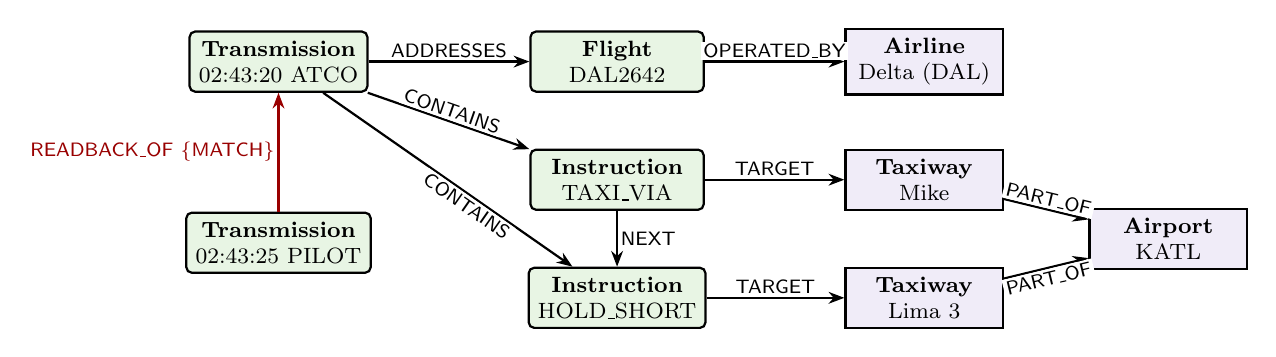
\begin{tikzpicture}[font=\footnotesize,
 dyn/.style={draw,thick,rounded corners=2pt,fill=comp,minimum height=0.75cm,minimum width=2.2cm,align=center},
 sta/.style={draw,thick,fill=res,minimum height=0.75cm,minimum width=2.0cm,align=center},
 e/.style={-{Stealth[length=2mm]},thick}, l/.style={font=\scriptsize\sffamily,fill=white,inner sep=1pt}]
\node[dyn] (t1) at (0,0) {\textbf{Transmission}\\02:43:20 ATCO};
\node[dyn] (t2) at (0,-2.3) {\textbf{Transmission}\\02:43:25 PILOT};
\node[dyn] (f) at (4.3,0) {\textbf{Flight}\\DAL2642};
\node[sta] (al) at (8.2,0) {\textbf{Airline}\\Delta (DAL)};
\node[dyn] (i1) at (4.3,-1.5) {\textbf{Instruction}\\TAXI\_VIA};
\node[dyn] (i2) at (4.3,-3.0) {\textbf{Instruction}\\HOLD\_SHORT};
\node[sta] (m) at (8.2,-1.5) {\textbf{Taxiway}\\Mike};
\node[sta] (l3) at (8.2,-3.0) {\textbf{Taxiway}\\Lima 3};
\node[sta] (ap) at (11.3,-2.25) {\textbf{Airport}\\KATL};
\draw[e] (t1)--node[l,above]{ADDRESSES}(f);
\draw[e] (f)--node[l,above]{OPERATED\_BY}(al);
\draw[e] (t1)--node[l,sloped,above]{CONTAINS}(i1);
\draw[e] (t1)--node[l,sloped,below,pos=0.6]{CONTAINS}(i2);
\draw[e] (i1)--node[l,above]{TARGET}(m);
\draw[e] (i2)--node[l,above]{TARGET}(l3);
\draw[e] (m)--node[l,above,sloped]{PART\_OF}(ap);
\draw[e] (l3)--node[l,below,sloped]{PART\_OF}(ap);
\draw[e,red!60!black] (t2)--node[l,left,text=red!60!black]{READBACK\_OF \{MATCH\}}(t1);
\draw[e] (i1)--node[l,right]{NEXT}(i2);
\end{tikzpicture}
\caption{KG 인스턴스 예시 (\S\ref{sec:data}의 실제 교환). 초록은 사건 계층으로 유효 구간·출처·신뢰도를 가지고, 보라는 정적 KB 계층이다.}
\end{figure}

%==========================================================
\section{Canonicalization: Callsigns \& Values}
%==========================================================
\begin{keybox}{슬라이드 요점}
\begin{itemize}[leftmargin=12pt]
\item \textbf{콜사인 해소:} \texttt{Alpha 265}, \texttt{Delta 265}, \texttt{265}처럼 서로 다른 표면형을 하나의 \texttt{Flight} 노드로 합친다. 판단 근거는 FAA 콜사인 표 \cite{faa7340}, 발음 유사도, \emph{그래프 문맥}(직후 복창, 최근 활성 항공편)이다 \cite{nigmatulina2022,itext2kg}.
\item \textbf{값·고유명사 정규화:} 표기 변이와 오인식을 표준형으로 바꾼다. 예: \texttt{Fox, shot}$\to$\cmd{Foxtrot}, \texttt{19-1}$\to$\cmd{119.1}, \texttt{line of ground}$\to$\cmd{Atlanta Ground}. 이어서 KATL 레이아웃의 실제 유도로·활주로 노드에 연결한다.
\item 연결에 실패하면 버리지 않고 \cmd{KB\_VIOLATION}으로 남긴다. 오인식인지 맥락 오류인지 사후에 추적할 수 있다.
\end{itemize}
\end{keybox}

\begin{center}
\begin{tikzpicture}[font=\footnotesize,
 m/.style={draw,thick,minimum width=2.4cm,minimum height=0.6cm,fill=white},
 c/.style={draw,thick,fill=blue!55!black,text=white,minimum width=2.2cm,minimum height=0.9cm,align=center},
 a/.style={-{Stealth[length=2mm]},thick}]
\node[font=\small\bfseries] at (0,1.0) {Before};
\node[m] (a1) at (0,0.2) {Alpha 265};
\node[m] (a2) at (0,-0.6) {Delta 265};
\node[m] (a3) at (0,-1.4) {265 (콜사인 생략)};
\draw[thick] (2.1,1.1)--(2.1,-1.9);
\node[font=\small\bfseries] at (4.6,1.0) {After};
\node[m] (b1) at (3.6,0.2) {Alpha 265};
\node[m] (b2) at (3.6,-0.6) {Delta 265};
\node[m] (b3) at (3.6,-1.4) {265};
\node[c] (f) at (7.0,-0.6) {\textbf{DAL265}\\{\scriptsize Flight}};
\draw[a] (b1)--(f); \draw[a] (b2)--(f); \draw[a] (b3)--(f);
\node[font=\scriptsize,align=left,anchor=west] at (8.3,-0.6) {근거: \texttt{Alpha}는 telephony 표에 없음,\\편명 일치, 직후 복창 \texttt{Delta 265}\\$\Rightarrow$ \cmd{ASR\_CORRECTED} 기록};
\end{tikzpicture}
\end{center}

\begin{addbox}
\textbf{KG가 STT를 돕는 되먹임.} 누적 그래프의 활성 콜사인과 유도로 이름을 다음 송신의 STT 프롬프트에 넣는다. 감시 데이터로 콜사인을 부스팅해 인식을 크게 개선한 선행연구 \cite{nigmatulina2022}를, 라벨 없이 쓸 수 있는 형태로 근사한 것이다. 이 고리 때문에 RQ2(``KG로 STT 오류를 교정할 수 있는가'')가 단순 후처리가 아니라 \emph{구조적 장점}이 된다.
\end{addbox}

%==========================================================
\section{Fusion: Cross-Speaker Corroboration \& Temporal Validity}\label{sec:fusion}
%==========================================================
\begin{keybox}{슬라이드 요점}
\begin{itemize}[leftmargin=12pt]
\item Team 2는 \emph{두 출처}(SEC·Wikipedia)에 같은 관계가 나오면 신뢰도를 올렸다(두 출처 일치 시 정밀도 94\%). 우리 도메인에서는 \textbf{관제사와 조종사가 독립된 두 출처}다. 지시와 복창의 개념이 일치하면 그 사실은 두 화자에게 \emph{교차 확인}된 것이다.
\item \textbf{신뢰도 등급}
  \begin{itemize}
  \item \textbf{HIGH}: 지시--복창 개념 일치
  \item \textbf{MEDIUM}: 한쪽 발화만 있음
  \item \textbf{LOW}: STT 신뢰도가 낮거나, 교정(\cmd{ASR\_CORRECTED})이 개입됨
  \end{itemize}
\item \textbf{시간 융합}: 상태형 지시는 유효 구간을 가지고, 대체되는 지시가 오면 삭제하지 않고 \emph{무효화}한다 \cite{zep2025}. 여러 주파수(Del$\to$Gnd$\to$Dep)의 송신을 UTC로 병합해 같은 항공편의 이관 흐름을 잇는다.
\end{itemize}
\end{keybox}

\begin{addbox}
\textbf{왜 이 신뢰도 정의가 타당한가.}
\begin{itemize}[leftmargin=12pt]
\item 복창의 목적 자체가 ``상대가 같은 내용을 이해했는지 독립적으로 확인''하는 것이다 \cite{faa7110}. 그래서 일치는 사실의 정확성에 대한 증거가 된다.
\item 반대로 \emph{불일치}는 두 가지로 해석될 수 있다. (a) 실제 복창 오류, (b) 한쪽의 STT 오류. 두 경우를 섞지 않도록 불일치 경보에는 STT 신뢰도와 교정 이력을 함께 붙인다. 이것이 Team 2의 ``evidence traceability''에 대응한다.
\item 이 정의는 \S\ref{sec:eval}에서 등급별 정밀도로 검증한다. 가설은 ``HIGH의 근거 정밀도가 MEDIUM보다 높다''이다.
\end{itemize}
\end{addbox}

\begin{center}
\begin{tikzpicture}[font=\footnotesize, x=0.62cm]
\draw[-{Stealth},thick] (0,0)--(20.5,0) node[right]{UTC};
\foreach \x/\l in {0.5/02:43:04,8.5/02:43:20,11/02:43:25} {\draw (\x,0.1)--(\x,-0.1) node[below,font=\scriptsize]{\l};}
\draw (12.5,0.1)--(12.5,-0.1) node[below=7pt,font=\scriptsize]{02:43:28};
\fill[green!25] (0.3,0.35) rectangle (2.3,0.75); \node[anchor=west] at (2.4,0.55) {PILOT: DAL2642 택시 요청 (information Papa $\to$ 맥락)};
\fill[blue!25] (8.4,0.95) rectangle (10.8,1.35); \node[anchor=east] at (8.3,1.15) {ATCO: DAL2642 TAXI\_VIA Mike, HOLD\_SHORT Lima 3};
\fill[green!25] (10.9,1.55) rectangle (12.3,1.95); \node[anchor=east] at (10.8,1.75) {PILOT: readback $\Rightarrow$ \textbf{MATCH / HIGH}};
\fill[blue!25] (12.4,2.15) rectangle (13.6,2.55); \node[anchor=east] at (12.3,2.35) {ATCO: \texttt{Delta 26-45} HOLD\_SHORT Lima 3 $\Rightarrow$ 유사 콜사인 판정 필요};
\fill[orange!70] (8.5,-1.05) rectangle (20.3,-0.8); \node[anchor=east,font=\scriptsize] at (8.3,-0.92) {$\tau$(HOLD\_SHORT Lima 3, DAL2642) = [02:43:20, 대체 지시까지)};
\end{tikzpicture}
\end{center}
{\footnotesize 네 송신 모두 KATL \cmd{Gnd-All} 실제 전사다. 유효 구간의 종료 시점은 이후 대체 지시로 정해진다.}

%==========================================================
\section{Quality Evaluation}\label{sec:eval}
%==========================================================
\begin{keybox}{슬라이드 요점}
\begin{itemize}[leftmargin=12pt]
\item 교수님 지침에 따라 KG의 대규모 정량 평가는 하지 않는다. 대신 \textbf{질적 평가를 주로 하고, 근거가 명확한 소규모 정량 점검}으로 품질을 입증한다.
\item \textbf{E1 역량 질문(CQ)}: 온톨로지가 답해야 할 질문을 먼저 정하고, KG가 답하는지 확인한다(질적, \cite{gruninger1995}).
\item \textbf{E2 근거 대비 정밀도 감사}: 관계 표본을 원음·전사와 대조한다(Team 2의 Precision에 대응).
\item \textbf{E3 주입 오류 탐지}: 복창 오류는 1\% 미만으로 드물다. 그래서 정상 복창에 통제된 오류를 주입해 탐지율과 오경보율을 잰다(Team 2의 Recall에 대응, \cite{helmke2022}).
\item \textbf{E4 RQ4 진단}: 한국·일본 교신에서 처음 실패한 모듈의 분포를 본다.
\end{itemize}
\end{keybox}

\begin{addbox}
\textbf{왜 평가를 보강했는가 (논리 공백 메우기).}
\begin{enumerate}[leftmargin=14pt]
\item ``평가 생략 + 데모''만으로는 데모 장면이 \emph{골라 뽑은 사례}라는 반론을 막기 어렵다. Team 2가 호평받은 지점도 문제정의를 \emph{입증}하는 단계였다.
\item 우리 도메인에는 Team 2의 ETO 같은 \textbf{외부 기준 데이터가 없다}. 그래서 재현율은 ``KG 사실 재현율''이 아니라 ``\emph{이상 상황 탐지 재현율}''로 재정의한다.
\item 실제 복창 오류는 1\% 미만이라 \cite{cardosi94} 5.5시간 데이터에 몇 건 없을 수 있다. 데모에서 오류 탐지를 보이려면 \emph{주입}이 필요하다. 인공 복창 오류 표본은 DLR 연구에서도 관제사 실험에 쓰였다 \cite{helmke2022}.
\item 품질 차원은 Linked Data 품질 서베이의 정의를 따른다 \cite{zaveri2016}.
\end{enumerate}
\end{addbox}

\subsection*{E1. 역량 질문 기반 질적 평가}
역량 질문은 ``온톨로지가 답할 수 있어야 하는 질문''으로 요구사항을 정의하고, 마지막에 이 질문들로 온톨로지를 검증하는 방법이다 \cite{gruninger1995,noy2001}. 판정 기준은 \emph{KG에서 질의로 답이 나오는가}(통과/실패)와 \emph{답에 근거 송신이 붙는가}이다.
\begin{center}\small
\begin{tabularx}{\textwidth}{@{}l>{\raggedright\arraybackslash}X l l@{}}
\toprule
CQ & 질문 & 관련 RQ & 필요 구조\\\midrule
CQ1 & DAL2642가 받은 지시를 시간순으로 나열하면? & RQ1 & \cmd{NEXT}, $\tau$\\
CQ2 & 02:40--02:50Z에 Lima 3에서 대기 지시를 받은 항공편은? & RQ1, RQ3 & \cmd{TARGET}, $\tau$\\
CQ3 & 복창이 없거나 콜사인 없이 복창된 지시는? & RQ3 & \cmd{READBACK\_OF}\\
CQ4 & 복창과 지시의 유도로·활주로가 다른 경우는? & RQ3 & 개념 비교\\
CQ5 & STT 교정이 개입된 콜사인과 그 근거 발화는? & RQ2 & \cmd{ALIAS}, prov\\
CQ6 & KATL에 존재하지 않는 유도로가 언급된 송신은? & RQ2 & 정적 KB 연결\\
CQ7 & Tower로 이관된 뒤에도 Ground 지시를 받은 항공편은? & RQ3 & \cmd{MONITOR}/\cmd{CONTACT} $\tau$\\
CQ8 & 지금($t$) 활주로 8R로 택시 중인 항공편은? & RQ3 & 스냅샷 $\G|_t$\\
\bottomrule
\end{tabularx}
\end{center}

\subsection*{E2. 근거 대비 정밀도 감사}
\begin{itemize}
\item \textbf{표본}: 관계 유형별 10개씩, 약 60--80개 (Team 2의 수동 감사 79개와 같은 규모).
\item \textbf{판정}: 사람이 원음 구간과 전사를 듣고 ``명시적으로 지지 / 부분 지지 / 지지 안 됨''을 단다. 선택적으로 LLM 판정을 보조 의견으로 붙인다(LLM-as-a-judge \cite{zheng2023judge}).
\item \textbf{보고}: 전체, 신뢰도 등급별(HIGH/MEDIUM/LOW), 관계 유형별 정밀도. 표본이 작으므로 \emph{Wilson 95\% 신뢰구간}을 함께 보고한다 \cite{wilson1927}.
\item \textbf{가설}: HIGH(교차 확인) $>$ MEDIUM $>$ LOW. 성립하면 \S\ref{sec:fusion}의 신뢰도 정의가 검증된다.
\end{itemize}

\subsection*{E3. 주입 오류 탐지 (복창 이상 재현율)}
정상(\cmd{MATCH}) 쌍 $N$개를 골라 복창 쪽 텍스트에 아래 변형 중 하나를 넣는다. 변형하지 않은 쌍은 오경보 측정용 대조군으로 남긴다.
\begin{center}\small
\begin{tabularx}{\textwidth}{@{}l>{\raggedright\arraybackslash}X l l@{}}
\toprule
유형 & 변형 예 & 근거 & 기대 판정\\\midrule
좌/우 혼동 & \texttt{8 right}$\to$\texttt{8 left} & 가장 흔한 실제 오류 \cite{cardosi94} & \cmd{MISMATCH}\\
유도로 치환 & \texttt{Lima 3}$\to$\texttt{Lima 4} & 대상 오해 & \cmd{MISMATCH}\\
콜사인 숫자 변경 & \texttt{2642}$\to$\texttt{2462} & 유사 콜사인 \cite{eurocontrol} & \cmd{MISMATCH} 또는 미연결\\
필수 항목 누락 & \texttt{hold short} 삭제 & 부분 복창 & \cmd{PARTIAL}\\
콜사인 누락 & 끝의 콜사인 삭제 & FAA §2-4-3 \cite{faa7110} & \cmd{NO\_CALLSIGN}\\
\bottomrule
\end{tabularx}
\end{center}
보고 지표는 유형별 탐지율(=재현율)과 대조군 오경보율이다. 텍스트 수준 주입은 STT 오류가 없는 \emph{상한}을 재는 것이다. 그래서 같은 쌍의 원음 기반 결과(오경보율)와 나란히 보고한다.

\subsection*{E4. RQ4 진단 (한국·일본)}
국가별 15--20개 송신에 정답을 달고 콜사인 인식률, 명령 개념 F1, \emph{처음 실패한 모듈} 분포를 보고한다. 조건은 (a) 그대로 적용, (b) 지역 자원만 교체 두 가지다. 일본은 LiveATC, 한국은 VATSIM(모의 교신이라는 점을 명시) 또는 허가된 실제 녹취를 로컬에서만 처리한다.

\subsection*{평가 결과 (KATL Ground 5.84\,h, 2026-10-14 실행)}
\begin{center}\small
\begin{tabularx}{\textwidth}{@{}l>{\raggedright\arraybackslash}X@{}}
\toprule
평가 & 결과\\\midrule
E1 역량 질문 & \textbf{8/8} 답변 가능·비어 있지 않음·원음까지 추적 가능. 예: CQ2 ``8R 대기 지시를 받은 항공편'' 12건, CQ8 시점 스냅샷 84건\\
E2 근거 정밀도 & \textbf{잠정} 60.0\% (95\% CI 47.4--71.4, n=60), 판정은 추출과 다른 모델(Qwen3.5-9B)로 했다. 신뢰도별로 HIGH 80\% (n=5) $>$ MEDIUM 66.7\% (n=24) $>$ LOW 50\% (n=8)로 가설과 같은 방향이다. 관계별로는 TARGET 83\%, ADDRESSES·VIA 67\%, INSTRUCTION\_TYPE 50\%, READBACK\_OF 33\%다. \emph{확인해 보니 LLM 판정이 명백한 일치도 기각하는 경우가 있어 수치가 불안정하다. 60행 시트에 사람 라벨을 단 뒤 다시 보고한다.}\\
E3 주입 오류 & 대조군 오경보 \textbf{0\%} (n=71, CI 0--5.1). 탐지율: 콜사인 숫자 변경 \textbf{95.5\%} (n=67), 콜사인 누락 \textbf{91.2\%} (n=57), hold short 누락 100\% (n=6), 유도로 치환 56.1\% (n=66), 좌/우 활주로 25\% (n=4). 규칙 추출기 기준선은 유도로 치환 90\%, 콜사인 97.6\%, 오경보 0\% (n=41)\\
E4 RQ4 & 정답 템플릿 20개 생성 (\texttt{data/gold/katl\_gnd\_gold\_template.jsonl}). 일본·한국 데이터 확보 후 같은 절차로 실행\\
\bottomrule
\end{tabularx}
\end{center}

\begin{addbox}
\textbf{결과 해석.}
\begin{itemize}[leftmargin=12pt]
\item \textbf{콜사인 관련 이상은 잘 잡는다}(91--96\%). 유사 콜사인이 사고 기여의 33\%라는 근거 \cite{eurocontrol}와 연결되는 강점이다.
\item \textbf{유도로 치환 탐지는 LLM(56\%)이 규칙 추출기(90\%)보다 낮다.} LLM이 복창에서 경로를 생략하면 비교 근거가 사라지기 때문이다. 결과적으로 정밀도와 탐지율 사이에 상충이 있고, 두 추출기를 함께 쓰는 하이브리드 설계의 근거가 된다.
\item \textbf{좌/우 활주로 혼동}은 지상 복창에 활주로가 직접 언급되는 경우가 드물어 표본이 4개뿐이다. Tower 데이터가 필요하다.
\item \textbf{주의:} 실제 MISMATCH 경보 20건 중 상당수는 추출 잡음으로 생긴 거짓 경보로 보인다(예: 경로 일부만 복창한 경우). 데모에서는 경보를 \emph{검토 대상}으로 제시하고, 근거와 원음을 함께 보여준다.
\end{itemize}
\end{addbox}

\paragraph{품질 차원 대응표 \cite{zaveri2016}.}
\begin{center}\small
\begin{tabular}{@{}lll@{}}
\toprule
품질 차원 & 우리 점검 & 해당 절\\\midrule
정확성 (accuracy) & 근거 대비 정밀도 감사 & E2\\
완전성 (completeness) & 역량 질문 통과 여부, 주입 오류 재현율 & E1, E3\\
일관성 (consistency) & 온톨로지 스키마·어휘 단서 검증 (구현은 SHACL 대신 코드 검사) & 온톨로지 절\\
적시성 (timeliness) & 유효 구간·무효화, 시점 스냅샷 질의 & Fusion, CQ8\\
추적성 (provenance) & 모든 사실에 원음 구간·전사 연결 & 전체\\
\bottomrule
\end{tabular}
\end{center}

%==========================================================
\section{KG Exploration: Application}
%==========================================================
\begin{keybox}{슬라이드 요점}
\begin{itemize}[leftmargin=12pt]
\item \textbf{제안 응용:} 지상 관제 \emph{상황 인식 보조}와 \emph{사후 안전 분석} QA.
\item \textbf{사용자:}
  \begin{itemize}
  \item 관제 감독자: 최근 10분간 복창 불일치 목록
  \item 안전 분석가: 사건 전후 특정 항공편의 지시 이력과 원음 근거
  \item 관제 교육생: 복창 패턴 피드백
  \end{itemize}
\item \textbf{예시 질문:} ``\emph{DAL2642가 Lima 3에서 대기하라는 지시를 받고 제대로 복창했는가?}'' $\to$ 지시 사건, 복창 판정, 신뢰도, 원음 구간을 함께 답한다.
\end{itemize}
\end{keybox}

\noindent\textbf{실제 KG의 질의 결과 (DAL2642).} 관제사는 콜사인을 번호만으로 불렀다(``2642, ... taxi via Mike, hold for the Lima 3''). M5가 직전 조종사 요청을 통해 이를 DAL2642로 해소했다. 조종사 복창(``Mike, hold short Lima 3, Delta 2642'')과 개념 단위로 비교한 결과는 \cmd{MATCH}이고, 두 지시 모두 신뢰도 \textbf{HIGH}(교차 확인)를 받았다. \texttt{hold for}는 \cmd{HOLD\_SHORT}로 정규화되었다. 같은 구간을 다른 실행에서 전사하면 \texttt{on the ground} / \texttt{Lender Ground}처럼 달라지는데, 이것이 \ch{C2}·\ch{C5}가 실제로 반복된다는 증거다.

\begin{figure}[h!]
\centering
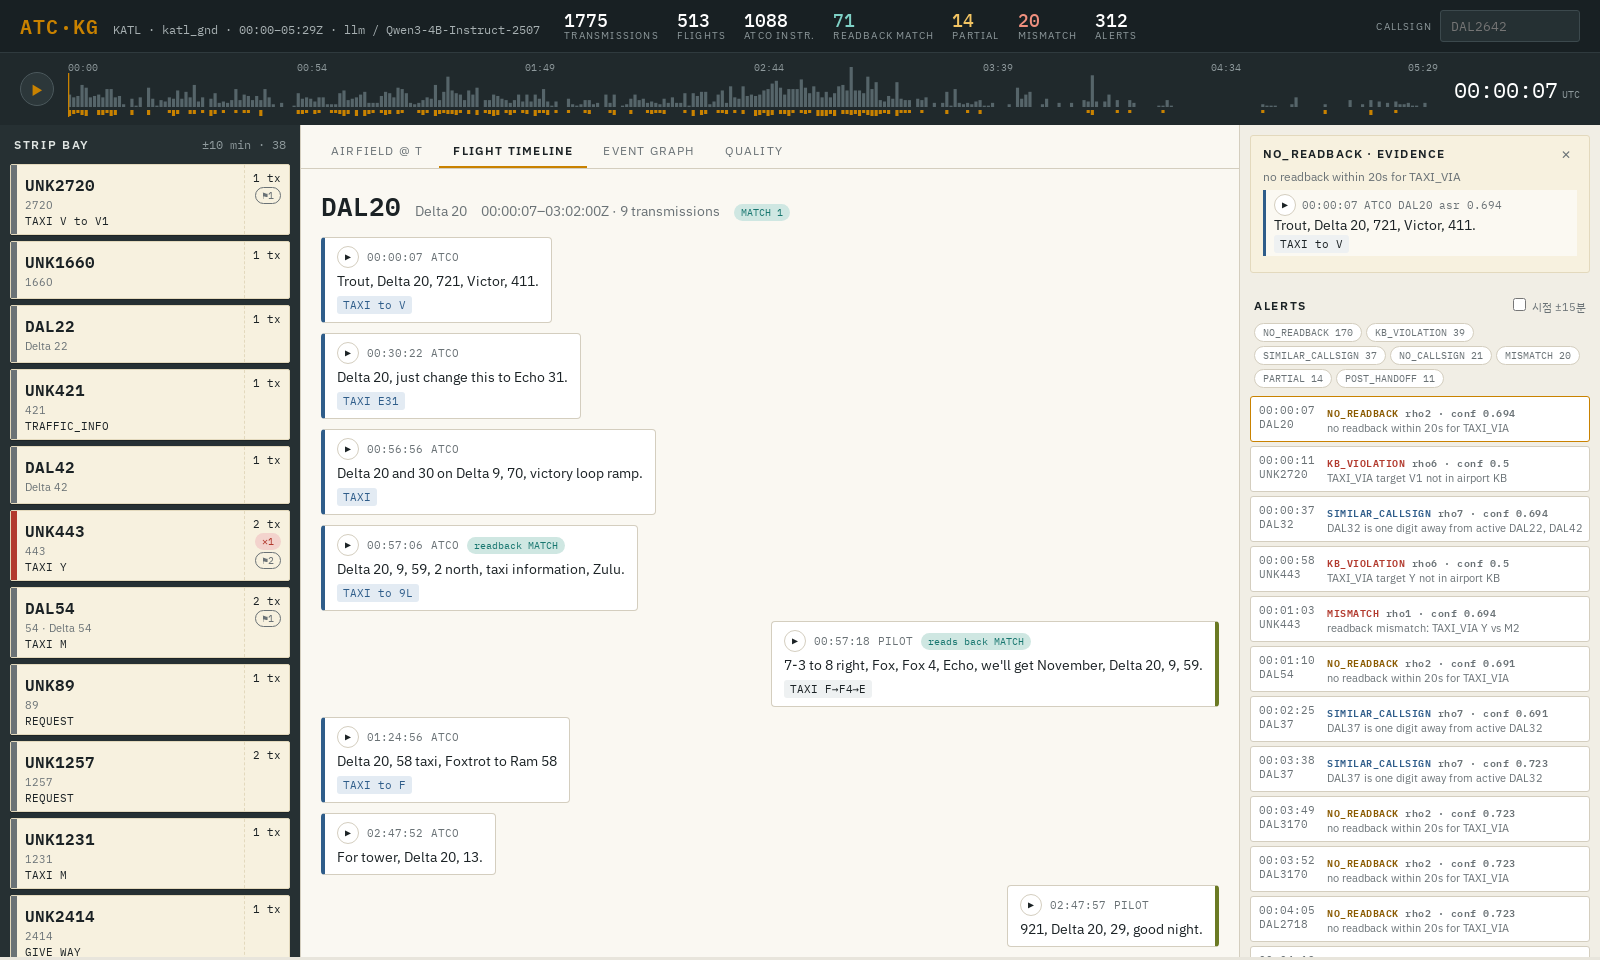
\includegraphics[width=\textwidth]{figures/demo_timeline.png}
\caption{웹 데모 (Flight timeline). 왼쪽은 시점 $t$ 주변 항공편의 flight strip, 가운데는 관제사(왼쪽)--조종사(오른쪽) 2열 교신 기록과 추출 개념, 오른쪽은 경보 목록과 근거 패널이다(원음 구간 재생 가능). 위쪽은 분당 송신 수와 경보를 보여주는 시간 스크러버다.}
\end{figure}

\begin{figure}[h!]
\centering
\begin{minipage}{0.49\textwidth}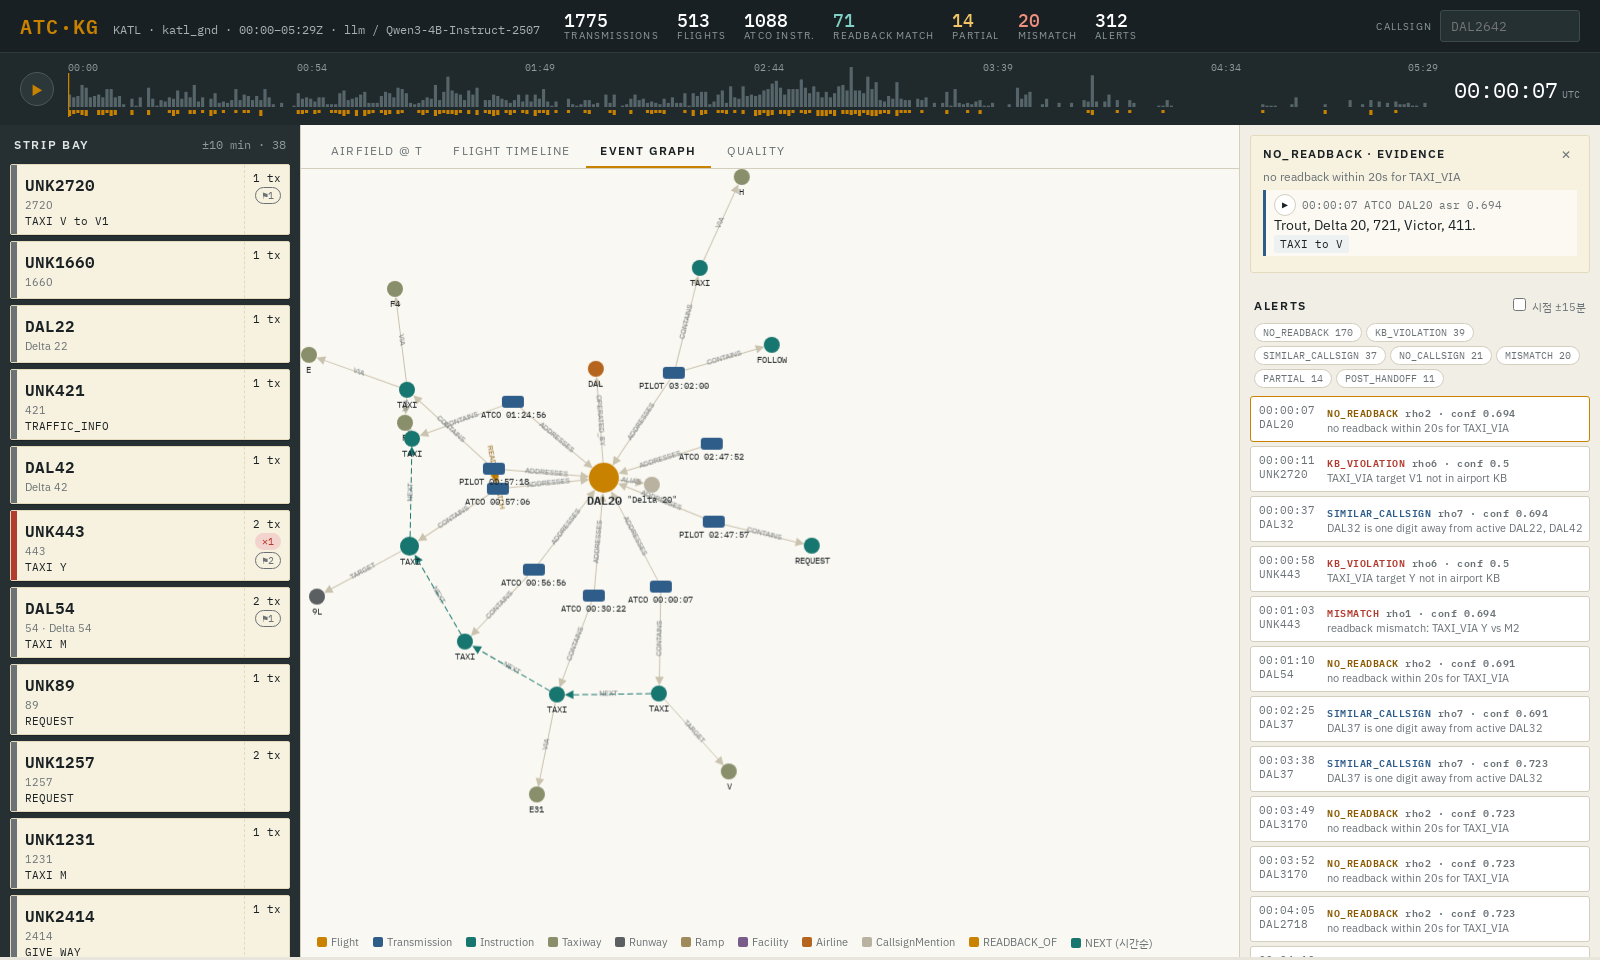
\includegraphics[width=\linewidth]{figures/demo_graph.png}\end{minipage}\hfill
\begin{minipage}{0.49\textwidth}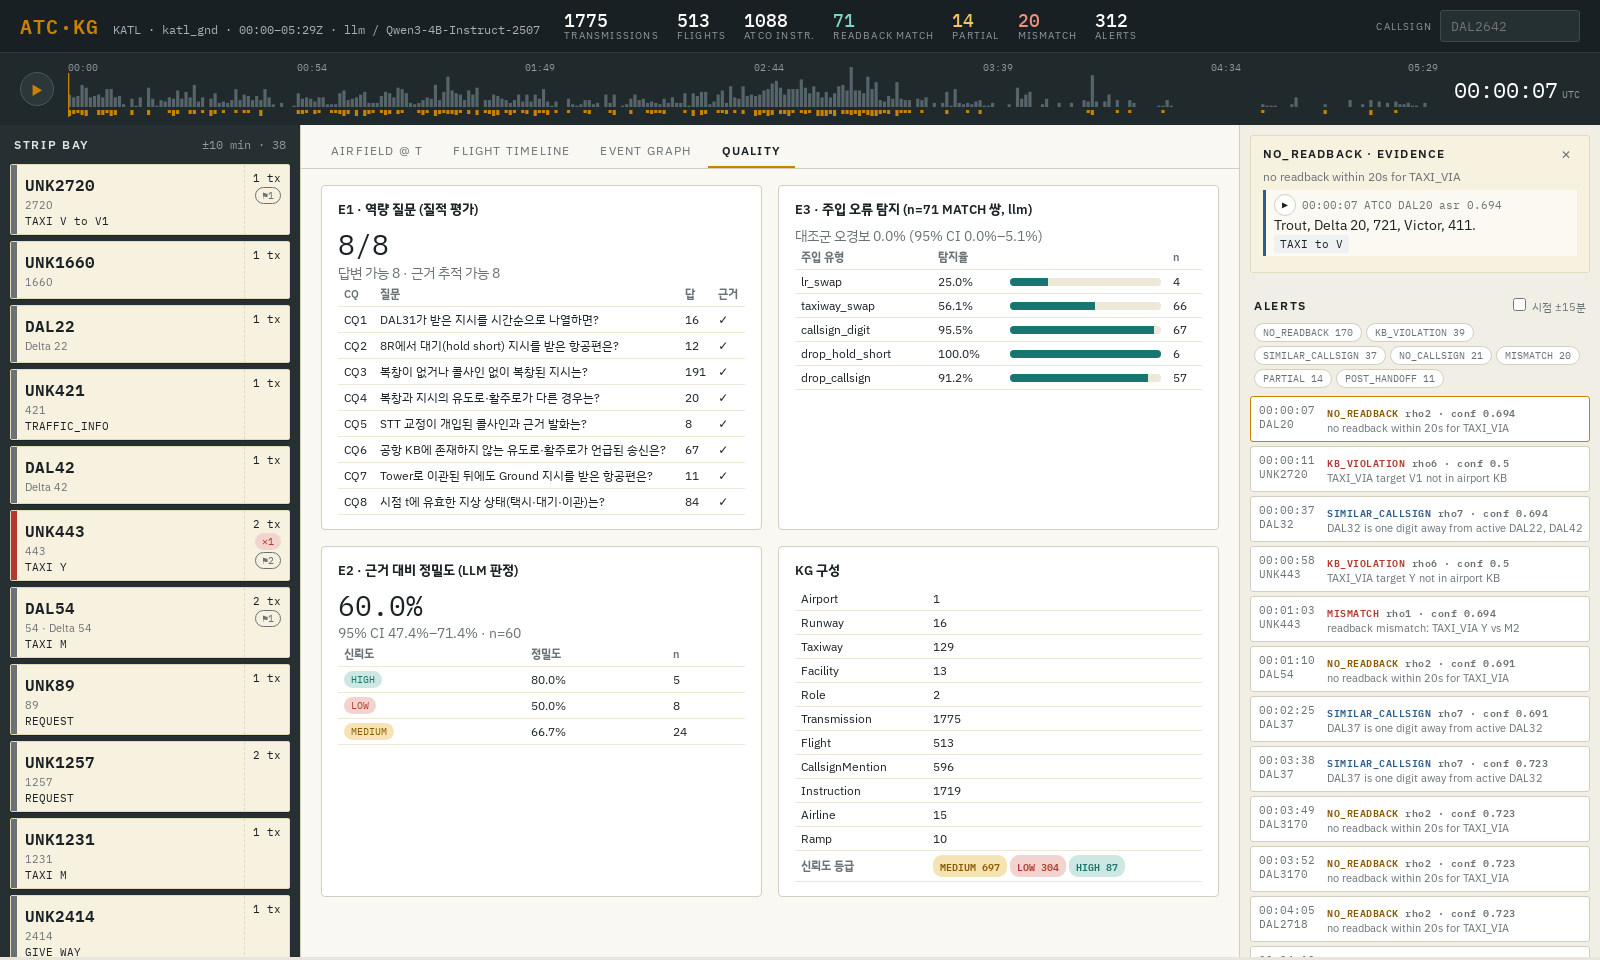
\includegraphics[width=\linewidth]{figures/demo_quality.png}\end{minipage}
\caption{왼쪽: 선택한 항공편의 사건 그래프(송신·지시·유도로, READBACK\_OF와 NEXT 간선). 오른쪽: 품질 탭(E1--E3 결과와 KG 구성).}
\end{figure}

\paragraph{Team 2 데모와의 차별점.} Team 2는 회사 네트워크 그래프와 근거 문장이 중심이다. 우리는 관제 현장의 \emph{flight progress strip} 은유를 쓰고, \textbf{시간축}(스크러버, 시점 스냅샷)과 \textbf{원음 근거 재생}을 중심에 둔다. Temporal KG라는 우리 문제의 핵심을 화면 구조에서 바로 보여주기 위해서다.

%==========================================================
\section{Conclusions}
%==========================================================
\begin{minipage}[t]{0.49\textwidth}
\textbf{Contributions (실측)}
\begin{itemize}[leftmargin=12pt]
\item 음성 교신을 입력으로 하는 \emph{사건 중심 Temporal KG}. 기존 ATM KG(정형 데이터)와 음성 복창 탐지(발화 단위) 사이의 공백을 잇는다.
\item 모든 사실에 원음 근거·신뢰도·유효 구간이 붙는다. 경보를 사람이 바로 검증할 수 있다.
\item 무료 공개 데이터, 학습 없는 파이프라인, 지역 자원 교체로 확장 가능한 구조(RQ4).
\item 5.84시간 실제 KATL 교신에서 항공편 513개, 관제 지시 1,088개, 복창 링크 105개를 구축했다. 주입 오류 탐지에서 콜사인 이상 91--96\%, 오경보 0\%.
\end{itemize}
\textbf{Takeaways}
\begin{itemize}[leftmargin=12pt]
\item 교차 확인(HIGH)의 정밀도가 가장 높았다(80\%, 잠정). Team 2의 ``두 출처 일치''와 같은 경향이다.
\item 관제사는 콜사인을 번호만으로 자주 부른다. 그래프 문맥(활성 항공편)으로 해소하는 단계가 필수다.
\item 고정 온톨로지와 정규화 단계가 있어야 개념 단위 비교가 가능하다.
\end{itemize}
\end{minipage}\hfill
\begin{minipage}[t]{0.49\textwidth}
\textbf{Limitations}
\begin{itemize}[leftmargin=12pt]
\item KATL Tower 부재로 착륙 허가 시나리오는 보조 데이터가 필요하다.
\item 하루치 일부(지상 5.84시간)와 STT 오류가 남는다. 실제 복창 오류는 드물어서 탐지 평가는 주입에 의존한다.
\item 해소되지 않은 콜사인(\texttt{UNK*})이 많고, 복창 링크는 관제 송신의 약 10\%에만 생긴다. 실제 MISMATCH 경보에 거짓 경보가 섞여 있다.
\item E2는 아직 LLM 판정(잠정)뿐이다. 사람 라벨이 필요하다.
\item 추출과 일부 판정이 LLM에 의존한다. 보안 자료는 로컬 LLM으로 제한된다.
\end{itemize}
\textbf{Next steps}
\begin{itemize}[leftmargin=12pt]
\item ADS-B(OpenSky) 결합으로 콜사인 해소와 위치 검증 강화.
\item Tower·Approach 피드 추가, 다중 주파수 이관 연결.
\item 한국 공역 확장(한영 혼용 처리, AIP Korea 정적 KB).
\end{itemize}
\end{minipage}

%==========================================================
\appendix
\section{논리 보강 내역}
\begin{center}\small
\begin{tabularx}{\textwidth}{@{}>{\raggedright\arraybackslash}p{3.8cm}>{\raggedright\arraybackslash}X>{\raggedright\arraybackslash}p{3.2cm}@{}}
\toprule
비어 있던 논리 & 보강 내용 & 근거\\\midrule
``왜 중요한가''의 최신 정량 근거 & FAA FY2023 활주로 침범 1,756건, A/B급 23건, 원인 비율 & \cite{faaincursion}\\
``왜 이 공항인가'' & KATL 세계 1위 여객·운항, Ground 지시--복창 밀집(실측) & \cite{aci2024}, \S\ref{sec:data}\\
콜사인 해소의 필요성 & 실측 콜사인의 88\%가 Delta, 3초 간격 유사 콜사인 사례 & \cite{eurocontrol}, \S\ref{sec:data}\\
평가 생략 시 데모의 대표성 & 역량 질문 질적 평가 + 소규모 근거 감사 & \cite{gruninger1995,noy2001,zaveri2016}\\
외부 기준 데이터 없음 (재현율 측정 불가) & 재현율을 \emph{이상 탐지 재현율}로 재정의하고 통제된 오류 주입 & \cite{helmke2022,cardosi94}\\
실제 오류가 드묾 & 주입 오류로 데모 시나리오 확보, 원음 기반 오경보율 병기 & \cite{cardosi94}\\
신뢰도 등급의 정당화 & 지시--복창을 독립 두 출처로 보는 교차 확인 정의 + E2 검증 가설 & \cite{faa7110}\\
작은 표본의 통계 & Wilson 95\% 신뢰구간 & \cite{wilson1927}\\
\bottomrule
\end{tabularx}
\end{center}

\begin{thebibliography}{99}\small
\bibitem{faa7110} FAA. \emph{Order JO 7110.65, Air Traffic Control}, §2-4-3 Pilot Acknowledgment/Readback.
\bibitem{faa7340} FAA. \emph{Order JO 7340.2, Contractions}.
\bibitem{faaincursion} FAA. Statement of Timothy L. Arel, COO Air Traffic Organization, U.S. Senate hearing (FY2023 runway incursion statistics). \url{https://www.faa.gov/testimony/statement-timothy-l-arel-chief-operating-officer-air-traffic-organization-hearing-united}
\bibitem{eurocontrol} Van Es, G. (NLR for EUROCONTROL). \emph{Air-Ground Communication Safety Study: Causes and Recommendations}, 2005.
\bibitem{cardosi93} Cardosi, K.~M. \emph{An Analysis of En Route Controller--Pilot Voice Communications}. DOT/FAA/RD-93/11, 1993.
\bibitem{cardosi94} Cardosi, K.~M. \emph{An Analysis of Tower (Local) Controller--Pilot Voice Communications}. DOT/FAA/RD-94/15, 1994.
\bibitem{prinzo2006} Prinzo, O.~V., Hendrix, A.~M., Hendrix, R. \emph{The Outcome of ATC Message Complexity on Pilot Readback Performance}. DOT/FAA/AM-06/25, 2006.
\bibitem{aci2024} Airports Council International. World airport traffic rankings 2024 (보도 기준: ATL 여객 약 1억 800만 명, 운항 1위).
\bibitem{bertraffic} Zuluaga-Gomez, J. et al. BERTraffic: BERT-based Joint Speaker Role and Speaker Change Detection for ATC Communications. \emph{IEEE SLT}, 2023.
\bibitem{helmke2025loss} Helmke, H., Clarke, S.~S., Ohneiser, O., Kleinert, M., Shetty, S., Kalyanam, K. Automatic Speech Recognition and Understanding in Air Traffic Control -- How Much Information Is Lost Over the Atlantic Ocean? \emph{DASC}, 2025. NASA NTRS 20250001345.
\bibitem{helmke2018} Helmke, H. et al. Ontology for Transcription of ATC Speech Commands of SESAR 2020 Solution PJ.16-04. \emph{DASC}, 2018.
\bibitem{kleinert2021} Kleinert, M. et al. Automated Interpretation of Air Traffic Control Communication: The Journey from Spoken Words to a Deeper Understanding of the Meaning. \emph{DASC}, 2021.
\bibitem{helmke2021} Helmke, H. et al. Readback Error Detection by Automatic Speech Recognition to Increase ATM Safety. \emph{14th USA/Europe ATM R\&D Seminar}, 2021.
\bibitem{helmke2022} Helmke, H. et al. Readback error detection (HAAWAII, Isavia 실데이터 81\% 탐지; 인공 복창 오류 표본을 사용한 관제사 실험). \emph{SESAR Innovation Days}, 2022.
\bibitem{chen2023} Chen, S. et al. Effects of Language Ontology on Transatlantic Automatic Speech Understanding Research Collaboration in the ATM Domain. \emph{Aerospace} 10(6):526, 2023.
\bibitem{keller2017} Keller, R.~M. \emph{The NASA Air Traffic Management Ontology}. NASA/TM-2017-219526, 2017.
\bibitem{keller2019} Keller, R.~M. Building a Knowledge Graph for the Air Traffic Management Community. \emph{Companion Proc. WWW}, 2019.
\bibitem{schrefl2022} Schrefl, M. et al. Creating an ATC Knowledge Graph in Support of the Artificial Situational Awareness System. \emph{Transportation Research Procedia} 64:328--336, 2022.
\bibitem{mekerishvili2025} Mekerishvili, A.~M., Sun, J., Jonk, P., de Vries, V. Structured Command Extraction from ATC Communications Using Open and Fine-Tuned Language Models. \emph{SESAR Innovation Days}, 2025.
\bibitem{scope2026} Deng, Q. et al. SCOPE: A Lightweight-training LLM Framework for Air Traffic Control Readback Monitoring. arXiv:2605.29543, 2026.
\bibitem{edc2024} Zhang, B., Soh, H. Extract, Define, Canonicalize: An LLM-based Framework for Knowledge Graph Construction. \emph{EMNLP}, 2024.
\bibitem{feng2024} Feng, X., Wu, X., Meng, H. Ontology-grounded Automatic Knowledge Graph Construction by LLM under Wikidata Schema. \emph{HI-AI@KDD}, 2024.
\bibitem{llmkgc2025} LLM-empowered Knowledge Graph Construction: A Survey. arXiv:2510.20345, 2025.
\bibitem{itext2kg} Lairgi, Y. et al. iText2KG: Incremental Knowledge Graphs Construction Using Large Language Models. \emph{WISE}, 2024.
\bibitem{atom2025} Lairgi, Y. et al. ATOM: AdapTive and OptiMized Dynamic Temporal Knowledge Graph Construction Using LLMs. arXiv:2510.22590, 2025.
\bibitem{zep2025} Rasmussen, P. et al. Zep: A Temporal Knowledge Graph Architecture for Agent Memory. arXiv:2501.13956, 2025.
\bibitem{naryw3c} Noy, N., Rector, A. (eds.) \emph{Defining N-ary Relations on the Semantic Web}. W3C Note, 2006.
\bibitem{knez2023} Knez, T., \v{Z}itnik, S. Event-Centric Temporal Knowledge Graph Construction: A Survey. \emph{Mathematics} 11(23):4852, 2023.
\bibitem{willard2023} Willard, B.~T., Louf, R. Efficient Guided Generation for Large Language Models. arXiv:2307.09702, 2023.
\bibitem{shacl} Knublauch, H., Kontokostas, D. (eds.) \emph{Shapes Constraint Language (SHACL)}. W3C Recommendation, 2017.
\bibitem{nigmatulina2022} Nigmatulina, I. et al. A Two-Step Approach to Leverage Contextual Data: Speech Recognition in Air-Traffic Communications. \emph{ICASSP}, 2022.
\bibitem{zuluaga2021} Zuluaga-Gomez, J. et al. Contextual Semi-Supervised Learning: An Approach to Leverage Air-Surveillance and Untranscribed ATC Data in ASR Systems. \emph{Interspeech}, 2021.
\bibitem{hfliveatc} nyuuzyou. \emph{LiveATC Recordings (Partial 2024-08-26)}. Hugging Face Datasets. LiveATC.net Terms of Use 적용.
\bibitem{atco2} Zuluaga-Gomez, J. et al. ATCO2 corpus. \emph{DMLR}, 2024. arXiv:2211.04054
\bibitem{uwbatcc} \v{S}m\'idl, L. et al. Air Traffic Control Communication (ATCC) Speech Corpora and Their Use for ASR and TTS Development. \emph{Language Resources and Evaluation} 53, 2019.
\bibitem{atcosim} Hofbauer, K., Petrik, S., Hering, H. The ATCOSIM Corpus of Non-Prompted Clean Air Traffic Control Speech. \emph{LREC}, 2008.
\bibitem{airbusatc} Pellegrini, T. et al. The Airbus Air Traffic Control Speech Recognition 2018 Challenge. \emph{Interspeech}, 2019.
\bibitem{atc0} Godfrey, J.~J. \emph{Air Traffic Control Complete} (ATC0). LDC94S14A, 1994.
\bibitem{tartan2025} Patrikar, J. et al. Image, Speech, and ADS-B Trajectory Datasets for Terminal Airspace Operations. \emph{Scientific Data}, 2025.
\bibitem{gruninger1995} Gr\"uninger, M., Fox, M.~S. Methodology for the Design and Evaluation of Ontologies. \emph{IJCAI-95 Workshop on Basic Ontological Issues in Knowledge Sharing}, 1995.
\bibitem{noy2001} Noy, N.~F., McGuinness, D.~L. \emph{Ontology Development 101: A Guide to Creating Your First Ontology}. Stanford KSL-01-05, 2001.
\bibitem{zaveri2016} Zaveri, A., Rula, A., Maurino, A., Pietrobon, R., Lehmann, J., Auer, S. Quality Assessment for Linked Data: A Survey. \emph{Semantic Web} 7(1):63--93, 2016.
\bibitem{zheng2023judge} Zheng, L. et al. Judging LLM-as-a-Judge with MT-Bench and Chatbot Arena. \emph{NeurIPS Datasets and Benchmarks}, 2023.
\bibitem{wilson1927} Wilson, E.~B. Probable Inference, the Law of Succession, and Statistical Inference. \emph{JASA} 22(158):209--212, 1927.
\end{thebibliography}
\end{document}
